\section{\'Etat de l'art}

Ce projet de deuxième année s'inscrit dans le contexte de la sécurité d'un système d'exploitation. La majeur partie des systèmes d'exploitation actuels ont intégré une forme de contrôle d'accès pour assurer un minimum de sécurité et de contrôle sur les activités des utilisateurs, dans le but de limiter les effets d'une attaque sur un système. Dans les faits, ce contrôle n'est pas suffisant et ne peut empêcher, par exemple, la compromission d'un système par l'intermédiaire d'un service possédant les droits d'administrateur \cite{TIOF}, ou l'échange d'informations par flux indirects, comme des fichiers temporaires.

Plus généralement, c'est dans l'absence de mécanisme de sécurité global imposé à un système que réside les manques des modèles de sécurité classique. Plus que simplement le noyau et les applications, ce sont l'ensemble des intéractions entre tous ces éléments qui doivent être contrôlées. Nous allons détailler les différents objectifs à atteindre avant de poursuivre sur les modèles théoriques et leur implémentation dans les systèmes d'exploitation modernes.

%  Nous allons détailler les objectifs à atteindre avant de présenter les différentes solutions disponibles.
% Il existe différents mécanismes qui permettent d'apporter des couches de sécurité à un tel système. Nous détaillerons donc les principes fondateurs de la sécurité pour enchaîner sur les solutions disponibles.

Nous allons réduire les concepts d'utilisateurs et d'applications aux ``simples'' processus qui sont la base de toute interaction avec un système. De même, les fichiers, sockets, les IPC sont autant d'éléments sur lesquels un processus peut agir et nous les regrouperons sous le terme d'objet.

\subsection{Les objectifs de sécurité}

La sécurité d'un système d'information et plus particulièrement la sécurité des systèmes d'exploitation réside dans l'application de mesures visant à atteindre les objectifs suivants :

\textbf{Confidentialité :}
Les informations ne doivent être accessibles qu'aux utilisateurs qui en ont besoin et qui disposent des privilèges correspondant. Il ne doit notamment pas être possible de transmettre de l'information confidentielle à un niveau inférieur.

\textbf{Intégrité :}
Le système reste dans un état cohérent. Les informations importantes comme les mots de passe, les binaires installés, les fichiers de configuration ne peuvent être modifiés par des utilisateurs non privilégiés.

\textbf{Disponibilité :}
Le système doit être réactif, stable et utilisable. Les programmes doivent pouvoir fonctionner correctement. Les contrôles de sécurité supplémentaires instaurés ne doivent pas limiter les capacités légitimes du système et des applications.

\textbf{Authenticité :}
Il est possible de savoir qui a effectué quelle action critique sur un système.

\textbf{Non-répudiation :}
L'origine et le contenu de certaines informations ne peut être mis en doute. Cela permet par exemple de s'assurer de l'enregistrement des comportements suspects sur une machine, ou de valider l'origine de certaines données.

\subsection{Le principe de séparation des privilèges}

Une des techniques utilisées pour tenter d'atteindre ces objectifs consiste à appliquer le principe de séparation des privilèges ou principe de moindre privilège. Il stipule qu'un programme (contrôlé ou non par l'utilisateur) ne doit disposer que des droits strictement nécessaires à son bon fonctionnement. Par exemple, il semble évident qu'un logiciel de traitement de texte n'a pas besoin d'avoir accès aux informations sensibles du système comme la liste des utilisateurs ou la liste des mots de passe.

L'application la plus courante de ce principe est la séparation entre les différents comptes sur un système. Une application lancée par un utilisateur ne bénéficie que des droits accordés à cet utilisateur.

\subsection{A qui faire confiance ?}

Il est possible d'employer différentes approches pour s'assurer de la sécurité d'un système d'exploitation, mais chacune d'entre elles repose à un moment ou un autre sur la confiance que l'on a dans l'un des éléments qui la constitue. On peut citer plusieurs cas de figures \cite{WCS}:

\begin{itemize}
  \item Faire confiance à tous les logiciels à propos du respect de la politique de sécurité, tout en étant conscient que les logiciels ne sont pas de confiance.% Trust all the software to abide by a security policy but the software is not trustworthy (this is computer insecurity).
  \item Faire confiance à tous les logiciels à propos du respect de la politique de sécurité et s'assurer que le logiciel est validé et fiable (analyse complète et exhaustive de tous les cas d'utilisations, de toutes les branches du code).% Trust all the software to abide by a security policy and the software is validated as trustworthy (by tedious branch and path analysis for example).
  \item Ne faire confiance à aucun programme, mais imposer une politique de sécurité même si la fiabilité de cette politique et son moyen d'application ne sont pas complétement assurés.% enforce a security policy with mechanisms that are not trustworthy (again this is computer insecurity).
  \item Ne faire confiance à aucun programme, mais s'assurer qu'une politique de sécurité est appliquée par des mécanismes matériels de confiance.% trustworthy hardware mechanisms.
\end{itemize}

Les modèles de sécurité standard se situent tous dans la première catégrie alors que les méthodes que nous allons présenter par la suite peuvent être placées dans les catégories trois et quatre. Le test complet de tous les logiciels présents sur un système d'exploitation est une tâche difficilement réalisable si l'on considère la diversité des matériels disponibles et la complexité d'une application telle que le noyau d'un système d'exploitation. Il existe des systèmes d'exploitation et plus particulièrement des noyaux certifiés critères communs, tel QNX\cite{QNX}, qui peuvent être classés dans la catégorie 2. En revanche, le code source de ces différents systèmes n'étant pas disponible librement, nous ne les détaillerons pas dans ce document.

\subsection{Les différentes méthodes de contrôle d'accès}

Pour atteindre les objectifs détaillés précédemment et assurer la séparation des privilèges, nous allons présenter dans cette partie plusieurs méthodes de contrôle d'accès.

\subsubsection{Contrôle d'accès discrétionnaire (DAC)}

Le contrôle d'accès discrétionnaire correspond à un modèle laissant à l'utilisateur, et donc aux programmes, tout contrôle sur les droits accordés aux objets qu'il possède. Un utilisateur peut ainsi compromettre un système en accordant des droits importants à d'autres utilisateurs sur les fichiers qu'il possède. Ce modèle ne permet pas d'assurer la confidentialité, l'intégrité d'un système. Il est à ranger dans la première catégorie des modèles qui font confiance aux logiciels sans imposer de contrôle de sécurité fort.

\subsubsection{Contrôle d'accès mandataire (MAC)}

Le contrôle d'accès mandataire repose sur la séparation entre les applications et l'entité prenant la décision d'autoriser ou d'interdire une action. Cette entité peut être implémentée au sein du noyau ou à l'aide de mécanismes externes au système, matériels \cite{ITXT}. Ce modèle permet d'assurer la conformité du système à un ensemble de règles qui forme une politique de sécurité. Il est ainsi possible d'appliquer le principe de moindres privilèges en partant d'une base n'autorisant aucune interaction puis en rajoutant progressivement des interactions autorisées. Le contrôle d'accès mandataire correspond aux catégories trois et quatre, où l'on ne fait pas confiance aux applications pour se reposer sur l'application d'une politique de sécurité plus ou moins fiable.

% \begin{figure}[h]
% 	\centering
% 	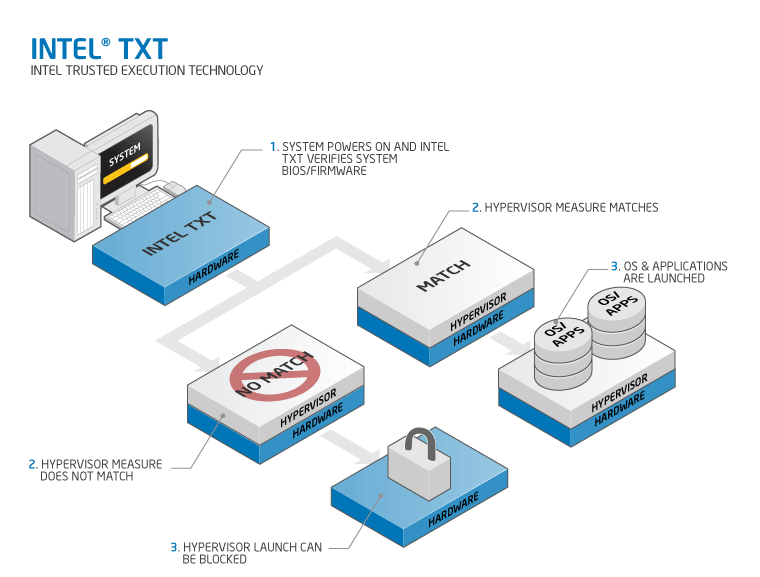
\includegraphics[scale=0.70]{attachements/techrefresh-info-txtfull.png}
% 	\caption{Intel Trusted Execution Technology}
% \end{figure}

\subsubsection{Sécurité multiniveau, multi catégorie (MLS ou MCS)}

Le modèle de sécurité multiniveau permet d'atteindre certains des buts fixés comme l'intégrité ou la confidentialité. Il repose sur la séparation des données en plusieurs domaines, imposant des règles limitant les interactions de l'utilisateur.

\textbf{Bell-LaPaluda :} Ce modèle préserve la confidentialité de l'information en n'autorisant un sujet à écrire uniquement dans un niveau de confidentialité supérieur ou égal, et à ne lire que dans un niveau de sécurité inférieur ou égal. Ce modèle présente plusieurs inconvénients majeurs parce qu'il ne permet pas d'imposer des contraintes d'intégrité et ne permet pas de faire de distinctions précises entre deux personnes possédant le même niveau d'accréditation.

\begin{figure}[h]
	\centering
	\includesvg{attachements/bell-lp}{0.45}
	\caption{Le modèle Bell-LaPadula}
\end{figure}

\textbf{Biba :} A contrario du modèle précédent, c'est l'intégrité qui est préservée, car seules les modifications dans un niveau de sécurité inférieur sont autorisées, et la lecture ne peut se faire que sur un niveau d'intégrité supérieur.

\begin{figure}[h]
	\centering
	\includesvg{attachements/biba}{0.45}
	\caption{Le modèle Biba}
\end{figure}

Ces deux modèles ne permettent pas d'atteindre plus d'un ou deux objectifs à la fois, et posent le problème de la sur-classification des données (toutes les données devenues confidentielles). Ceci conduit à l'introduction d'une méthode de dé-classification, compromettant l'ensemble du modèle.

\subsubsection{Contrôle d'accès basé sur des rôles (RBAC)}

Plus qu'un modèle réel de contrôle, c'est un modèle d'administration permettant de simplifier le travail de l'administrateur d'un système utilisant un contrôle mandataire. Le principe du contrôle d'accès mandataire consiste à attribuer des rôles à chaque utilisateur de la machine. Ces rôles donnent ainsi accès à différents éléments du système. Par exemple, les rôles d'utilisateur, d'administrateur et de webmestre peuvent être définis et un utilisateur classique pourra se voir attribuer le rôle de webmestre lui autorisant de modifier les pages disponibles sur un serveur sans avoir besoin de donner un accès administrateur complet à cette personne.

\subsubsection{Application de règles de politiques securité par les types (Type Enforcement)}

Ce principe repose sur l'association d'un contexte de sécurité à chaque objet et processus. L'accès à un object par un processus doit correspondre à une règle de la politique de sécurité pour être autorisé. Ce modèle nécessite l'attribution d'un contexte de sécurité à tous les objets du système, y compris les fichiers présents sur les supports de stockage.

\subsection{Solutions disponibles}

Nous allons détailler les implémentations de ces modèles de sécurité dans certains systèmes d'exploitation, notamment les systèmes ``libres'', pour lesquels nous pouvons avoir accès au code source : Linux et la famille des BSD.

\subsubsection{SELinux}

SELinux est une implémentation d'un mécanisme de contrôle d'accès mandataire basé sur le ``type enforcement'', de niveaux de sécurité/confidentialité non prédéfinis, et d'un contrôle d'accès basé sur les rôles. SELinux a été développé par la National Security Agency (NSA) et a été intégrée au noyau Linux une fois que l'architecture des Linux Security Modules fut mise en place. SELinux permet de contrôler pour chaque appel système la validité de l'interaction par rapport aux définitions d'une politique. On associe à chaque objets et processus un context de sécurité. L'accès à un object par un processus doit correspondre à une règle de la politique SELinux pour être autorisé. Il faut noter que chaque décision est prise indépendamment des précédentes : SELinux n'as pas de mémoire des transitions effectuées sur un système. C'est cette limitation et la possibilité d'utiliser les flux d'informations indirects, donc non contrôlés par SELinux, qui ont poussé la création de PIGA.
\begin{list}{}{}
 \item \textbf{Contrainte pour l'administrateur :} Il faut décrire la totalité des interactions possibles pour chaque programme présent sur un système. Il faut s'assurer du bon fonctionnement de ces politiques. Il n'existe pas d'outils pour valider les politiques SELinux. Seuls certains systèmes de fichiers supportent les attributs étendus nécessaires à la labelisation des fichiers présents sur les supports de stockage.
 \item \textbf{Avantages :} Séparation fine des privilèges et des rôles, intégrée dans le noyau. Des politiques ont déjà été écrites. Il existe une distribution facilitant le déploiement de ce type de protection : Fedora.
\end{list}

\subsubsection{PIGA}

L'ensemble désigné sous le nom de PIGA est le résultat de la thèse de Jérémy Briffaut ainsi que des contributions de l'équipe SDS du LIFO, et des étudiants de l'ENSIB. Il est constitué notamment d'une sur-couche à SELinux permettant de définir et imposer des propriétés de sécurité à l'échelle du système en plus des contrôles au niveau des interactions effectués par SELinux. Il apporte une ``mémoire'' à SELinux. Un tel résultat est obtenu après génération du graphe complet des interactions possibles et autorisées par une politique SELinux, recherche de chemins interdits, et consignation de ces chemins. Cette solution permet un contrôle plus avancé sur les flux d'informations dans un système, qu'ils soient directs ou indirects.
\begin{list}{}{}
 \item \textbf{Contrainte pour l'administrateur :} Connaissance du langage de définition de propriété PIGA, maîtrise préalable de SELinux, pré-requis matériels pour la ``compilation'' des politiques.
 \item \textbf{Avantages :} Un contrôle très fin sur les interactions dans un système, restriction (statique) des privilèges maximale.
\end{list}

Le système d'exploitation PIGA-OS basé sur la recherche effectuée sur PIGA a été vainqueur du concours Sec\&Si organisé par l'Agence Nationale pour la Recherche (ANR) \cite{PIGA}\cite{PIGA2}.

\subsubsection{grsecurity \& PaX}

\textsc{grsecurity} est une autre implémentation des mécanismes de contrôle d'accès mandataire et des listes de contrôle d'accès. Il permet aussi une gestion des droits basée sur les rôles. Souvent associé à \textsc{grsecurity}, PaX est un patch pour le noyau Linux ajoutant des restrictions et des contrôles sur les accès à la mémoire.
\begin{list}{}{}
 \item \textbf{Contrainte pour l'administrateur :} Certains programmes ne fonctionnent plus avec les restrictions implémentées par PaX. Il faut organiser correctement les binaires car la labellisation est effectuée par rapport à l'arborescence
 \item \textbf{Avantages :} Protection avancée de l'utilisation de la mémoire avec PaX (pile non exécutable, ...), fonctionnement un peu plus simple que SELinux
\end{list}

\subsubsection{TrustedBSD}

Le projet TrustedBSD consiste à intégrer à FreeBSD des fonctions de sécurité telles que les attributs étendus pour le système de fichier UFS2, les listes de contrôle d'accès, des capacités d'audit liées à la sécurité, plusieurs méthodes de contrôles d'accès mandataire.

\subsubsection{iptables}

Iptables et un logiciel permettant de contrôler plus facilement netfilter, le pare-feu intégré au noyau Linux. Il permet entre autre de définir précisément quels ports et quelles interactions avec le réseau sont autorisés sur une machine. Les règles iptables peuvent être modifiées dynamiquement pour autoriser ponctuellement une application à communiquer avec l'extérieur mais le comportement d'iptables est statique par défaut. Iptables est un pare-feu à états, c'est-à-dire qu'il garde en mémoire les interactions précédentes pour déterminer la légitimité des interactions suivantes.
\begin{list}{}{}
 \item \textbf{Contrainte pour l'administrateur :} Il faut préciser de manière exhaustive les ports utilisés sur une machine.
 \item \textbf{Avantages :} Contrôle fin des connexions réseaux possibles. Audit des connexions facilité.
\end{list}

\subsubsection{PIGA-SYSTRANS ou contextd}

Contextd est un démon chargé de coordonner différents mécanismes de sécurité sur un système Linux. En effet, dans toutes les solutions décrites précédemment, les programmes se voyaient attribuer les droits dont ils avaient besoin, pour toujours. Une application utilisant ponctuellement le réseau se voyait attribuée le droit définitif d'utiliser un port. Contextd introduit la notion de domaine (web, impôts, ...) lié à une activité particulière de l'utilisateur. Les programmes surveillés n'ont le droit de faire que ce qui leur est autorisé dans le domaine courant.
\begin{list}{}{}
 \item \textbf{Contrainte pour l'administrateur :} Maîtrise de SELinux, PIGA. Rédaction et test des règles exhaustives pour faire fonctionner les programmes avec contextd. Certains programmes nécessitent des modifications, surtout lorsque ceux-ci ont un comportement inter-domaine.
 \item \textbf{Avantages :} Presque la plus fine implémentation du principe de moindre privilèges.
\end{list}

% Pax = sécurité automatique
% SELinux, GrSec = MAC qui contrôle les accès directs
% PIGA = contrôle les accès indirects
% iptables contrôle le trafic réseau
% 
% contextd = chef d'orchestre + changement dynamique des règles des autres  mécanismes de protection pour adapter les permissions au domaine d'utilisation.
% 
% Chercher tous les systèmes de MAC/DAC/RBAC,...
% 
% Classer les MAC en fonction du travail à faire par l'administrateur ? en fonction d'où ils agissent ? par rapport à la logique interne (stateless ou statefull) ?
